\chapter{System Design}
\label{chap:3}

In this chapter, the overall system design is discussed. The chapter is divided up into 
nine sections with each section focusing on a different aspect of the complete
system. These nine sections are:

\begin{enumerate}
  \item The VM central controller.
  \item The Near Field Communication controller.
  \item The Quick Response Code camera.
  \item The product dispensing mechanism.
  \item The VM unit.
  \item The web server.
  \item The encryption scheme used.
  \item The security schemes used. 
  \item The transaction process for each payment option. 
\end{enumerate}

Each section explains which technology or service was used in the final
component design.

Where two or more available services or technologies were available,
a brief discussion and explanation is given as to why the particular technology or
service was used in the final design of the VM.

\section{System Overview}

Fig. \ref{fig:system-overview-pi} gives a diagrammatical layout of the complete system.
It shows the data interactions between the different sub-components of the complete
system.

\begin{figure}
\centering
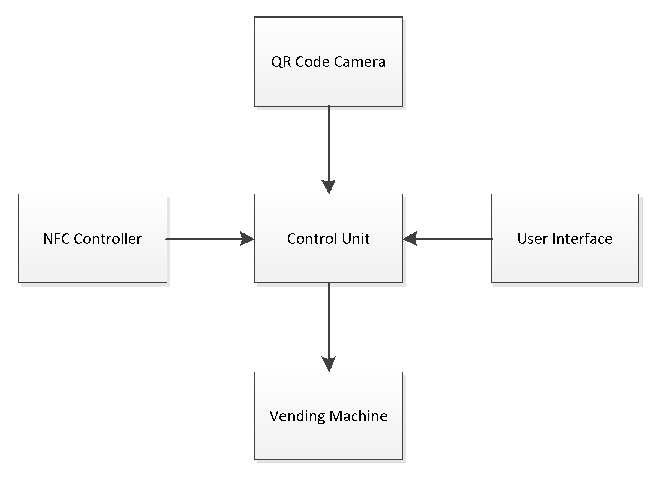
\includegraphics[clip=true, trim = 100 90 0 200, scale=0.7]{pi_system_overview}
\caption{System overview from the control unit's perspective.}
\label{fig:system-overview-pi}
\end{figure}

The components used in these subsystems are discussed in the subsequent sections of this
chapter.

\section{Central Control Unit}

To be able to handle the data processing that Quick Response (QR) Code decoding
and Near Field Communication (NFC) requires, a fairly powerful central controller
is required. The two controllers  that were considered for this project is the Raspberry
Pi microcomputer and the Arduino Uno microcontroller. These controllers are discussed in
this section. Their specifications are given in Table \ref{tab:arduino-raspi-specs}.

\subsection{Arduino Uno}

The Arduino Uno is popular open-source microcontroller. It is based on an 8-bit
Atmel ATmega328 ARM microprocessor.

\begin{table}
\footnotesize
\centering
\caption[Comparison between Arduino Uno and the Raspberry Pi Specs.]{Comparison between
Arduino Uno and the Raspberry Pi Specs [\cite{manual:arduino-specs},
\cite{website:raspi-specs}].}
  \begin{tabular}{|l|l|l|}
  \hline
    \textbf{Specification Detail} & \textbf{Arduino Uno} & \textbf{Raspberry Pi}
    \\\hline\hline Operating Voltage & 5 V & 3.3 V \\\hline
    Processor & Atmel ARM \@ 16 MHz &  ARM 6 \@ 700 MHz \\\hline
    GPIO Pins & 14 & 28 \\\hline
    Memory & 32 kB Flash & 512 MB RAM\\\hline
    Communication & i$^2$c, UART, SPI & SPI, UART, USB, i$^2$c, Ethernet \\\hline
    Price & R310.00 & R400.00 \\\hline
    Video Output & N/A & HDMI \\\hline
  \end{tabular}
  \label{tab:arduino-raspi-specs}
\end{table}

Because of its open-source design, there are a multitude of peripheral devices and expansion
boards (known as `shields'), along with all their libraries and drivers,
available locally. The Arduino's programming language of choice is a modified version of
C and comes with its own Integrated Development Environment. This, along
with its relatively low cost and specifications, made the Arduino Uno
an attractive option for this project.

\subsection{Raspberry Pi}
\label{sec:raspi}

The Raspberry Pi is a Linux-based microcomputer, designed and manufactured by the
Raspberry Pi Foundation in the UK for the purpose of educating and familiarising young
children with programming. However, its low price and respectable specifications makes it
a strong choice as a control unit for the VM.

The Pi was designed with the focus on Python as its main programming language, which makes
running scripts and controlling the board relatively simple. It also runs on a modified
version of Debian Linux, called Raspbian.

\subsection{Design Choice}

The Raspberry Pi was chosen as the central controller of this project and
controls the hardware connected to it via a Universal Serial Bus (USB) connection, or one of
its General Purpose Input Output (GPIO) pins.

The Pi was chosen ahead of the Arduino, because of its video stream processing
capabilities and that libnfc can be installed on it. This allows the Pi to decode QR
Codes and to communicate with an NFC-enable cellphone through an NFC add-on chip.
Furthermore, the Pi can interface with desktop peripheral hardware, such as a mouse and
keyboard, which made development and prototyping much simpler.

After development and optimisation has been completed for this project, work can begin on
porting it to a micro-controller, such as an Arduino. However, for the development phase
of this project, the Pi is a much better suited platform.

\section{NFC Controller}
\label{sec:nfc-controller}

The NFC controller that was used is the PN532 NFC shield from Adafruit Industries
[\cite{website:adafruit-nfc}]. It is based on the Phillips PN532 chip. 

The main reason it
was selected instead of other NFC controllers was that it has a large support base in the
open-source community and is fully compatible with the libnfc open-source NFC library
[\cite{website:libnfc-hardware}]. The manufacturer also provides
comprehensive documentation and guides on how to set up and configure the controller
[\cite{website:adafruit-tutorial}] for a Raspberry Pi.
 
The main purpose of this component is to add the option of sending or receiving data
through an NFC connection. This component is also capable of reading Radio
Frequency Identification (RFID) cards, such as student or staff cards, since NFC and RFID
transmit similar types of data. This adds the option of paying for the products with any
NFC-capable smart phone running Google's Android operating system, or with a Stellenbosch
University (SU) staff or student card.

\section{QR Code Camera}
\label{sec:webcam}

To decode QR Codes, the VM needs to take pictures of a code so that it can be
decoded by a QR Code library, such as the ZBar library. A PlayStation 2 EyeToy was
chosen and added to the system to facilitate this. It was chosen because its drivers are
freely available for Linux systems [\cite{website:webcam-drivers}], it interfaces easily
with the USB ports on the Pi and one was readily available for use.

There is currently a camera add-on available for the Pi, but this is relatively
expensive (approximately \$30 [\cite{website:raspi-camera}] versus the Pi's cost of \$35 
and the PS2 EyeToy's cost of \$10) and unavailable in locally at the time of writing.

\section{Product Dispensing}

\subsection{Coils}

To be able to effectively dispense bought products to the user, a coil mechanism is
used. These mechanisms are familiar and simple methods of dispensing goods.

These coils are designed and made in such a manner that one rotation of the coil will drop one
product. The turning motion is made by attaching a DC motor to the base of the coil.

\subsection{DC Motors}
\label{sec:dc-motor}

The motors attached to the base of the coils are two 12 V DC motors from Faulhaber
[\cite{manual:dc-motors}]. Although these motors are rated for 12 V, it is possible to run them
from a lower voltage. This will cause the motor to turn slower, and therefore be easier to
control. The motors are switched on by a 12 V relay switch controlled by the Raspberry Pi.

\subsection{Relay Switch}
\label{sec:relay-switch}

A relay is an electronic switch, which requires a voltage across it to open or close it.
With this, it is possible to control when the DC motors turn (after a successful
transaction) and when they are standing still.

The relays used here are 12 V, because they were readily available, but he Raspberry 
Pi can only deliver a maximum voltage of 5 V. Therefore, it was required that the
relay will be permanently connected to a 12 V DC supply. The relays are then switched by a
2N2222 transistor, which is controlled directly from the Pi's GPIO pins (see Sec.
\ref{sec:detail-switch} on p.\pageref{sec:detail-switch} for a detailed discussion on the
switch). This allows the Pi to directly control the motors and due to the circuit's
construction, the Pi is protected from the relatively high voltages and currents involved
in the working of the motor and relay.

\section{Vending Machine Unit}

The VM unit houses all the components (i.e. the Raspberry Pi, the NFC Shield,
webcam, switches, motors and the product coils). See Appendix \ref{app:vm-tekeninge} 
for detailed manufacturing drawings and a picture of the VM.

\section{Web Server}

A web server in the computing cloud is used to process and authenticate the
transactions that take place in the VM. This is done by
using a user database that is populated with the customers' login details that
they supply when they sign up for the VM service. The database
stores the customers' information, such as the customers' username, password and their
remaining balances. Part of the transaction process is to check if a customer has enough
credits loaded onto his account.

Arguably, the transaction authentication could have been done by the VM itself. However,
using a web server allows the system to be expanded beyond a single VM and
standardises the transaction process for all of the VMs connected to the server.

The server communicates with a customer through the customer's cellphone,
which sends data to the server over the internet via Hypertext Transfer Protocol
(HTTP) requests and Universal Resource Locators (URLs). How the web server is used to
process and authenticate each payment method is described in Sec. \ref{sec:transaction}.
 
\section{Encryption Scheme Design}

To prevent the system from being hacked, an asymmetric encryption scheme was
implemented. The main reasons for this choice is that the keys are easily
distributed, the encryption scheme is relatively secure and there is powerful
software available to encrypt the data exchanges.

The keys were generated using the PyCrypto module and were are hard-coded
into the VM and the web server during development. If required, old
keys can be replaced remotely over the internet or by a technician working on the
VM. The Android application has its own key. This key is distributed with the
application. 

The keys are hardcoded to keep the keys more secure and to avoid having to dynamically
update and redistribute the keys after each transaction.

Two different schemes were implemented for the Android NFC application and the
QR Code payment option. These two schemes are discussed in this section.

\subsection{Android NFC Application}

For the Android NFC application, a 1024-bit key based on the RSA encryption algorithm was
used. A 1024-bit key was chosen because it gives a good balance between security and
encryption speed. It was decided to base the application's encryption on RSA, because it
is already included in the Android Development Kit and is therefore the simplest to
implement and distribute with the application.

\subsection{QR Code}

For the QR Code payment option, a 384-bit key based on the ElGamal algorithm was
used. The reason for choosing this key size was to produce smaller, less complex
output which leads to a more readable QR Code. A simpler, more readable QR Code
takes less time to scan. A smaller key size also reduces the time it takes to
encrypt a data string.

It was also found that the RSA module in PyCrypto has a minimum key-length of 1024
bits, which is too long. The ElGamal module allows for key sizes of any bit
length, as long as it is longer than the string being encrypted. Therefore, ElGamal was
selected. 

\section{Security Scheme}
\label{sec:security-code-scheme}

In addition to the asymmetric encryption used on all data transfer to and from
the server to its clients, two more layers of security were added. The effectiveness of
these additional layers of security still rely upon the encryption scheme staying intact.
However, these extra security layers help to obscure the plain text message being
encrypted, thereby making it harder for would-be hackers to realise they have cracked the
encryption. It also prevents the same code from being used more than once without being
paid for. These security schemes are discussed in this section. 

\subsection{Random Character String}

The code transmitted to the server is a random 16-character hexadecimal string. The
product code 4 hex characters long and is embedded inside this 16-character string.
The product code is saved on the database and can therefore not be random. 

A hexadecimal string was chosen because it is a common data representation
format and it will make it harder for a hacker to see that they have
successfully broken through the security. For example, if the hackers manage to
break through the security, they will see a string like this one, A2FB32E1CFF7. If the
product code were alphanumeric, for example `coke\_350ml', the hackers will immediately
see that they have broken through. This scheme does not make the code uncrackable, but it
does make brute-force attacks harder to execute properly.

\subsection{Challenge and Response Code}
\label{sec:challenge-response}

To prevent customers from repeatedly using the same QR Code to buy a
product, a second layer of security was added. This layer is a
challenge-response scheme. 

Such a scheme works by having party A generate a
challenge (this can be a string or a number) and send it to party B. Party B then takes
this challenge and puts it through a previously agreed-upon process, e.g. puts the string
though a one-time hash or adds the numbers together. This is the response.
Party B then sends the back the response to party A, which then checks to see
if it is a valid response to party A's original challenge.

In the case of the VM, a 16 character hex string is being generated. It was decided to use
4 characters of the 16-character string, excluding the 4-character product code, as the
VM's challenge. After receiving this challenge, the server then takes out the agreed-upon
4 characters and embeds it inside the server's response code. When the VM scans the
customer's response QR Code, the VM checks to see if the 4 character response was part of
its original code the VM generated. This ensures that each code only dispenses one
product, because the 4 characters used are randomly generated and are therefore only
valid for one transaction.
 
\section{Transaction Design}
\label{sec:transaction}

Three different transaction processes were designed to accommodate for QR Code NFC and
RFID payments. However, all three of the payment options have some common elements to
them.

Firstly, each product in the VM is assigned a unique, 4-letter hexadecimal number. This is
done to comply with the security code scheme discussed in Sec.
\ref{sec:security-code-scheme}. When a customer selects a product to buy, this unique
code is used identify which product to dispense. To simplify the demonstration system,
only two codes are used. The second common element between the payment
options is that all the transactions require authentication from the central server. At
this stage, this excludes RFID card payments. The reason for this is explained in Sec.
\ref{sec:su-card}.

\subsection{QR Code Transactions}

The QR Code transaction process and the interactions between the different
system components is described diagrammatically in Fig.
\ref{fig:vm_prog_interaction}.

\begin{figure}
 \centering 
 \includegraphics[clip=true, trim = 60 430 0 140, scale=0.7]{qrcode_processflow_user}
 \caption{The VM QR Code transaction process.}
 \label{fig:vm_prog_interaction}
\end{figure}

Fig. \ref{fig:vm_prog_interaction} shows that the transaction begins with
the customer selecting a product to buy from the VM Graphical User
Interface (GUI). The VM then generates a QR Code which the customer scans. The QR Code
contains a URL that contains a link to the web server and the encrypted product data, the
VM's signature and the challenge-response code (the challenge-response scheme is
described in Sec. \ref{sec:challenge-response} on p.\pageref{sec:challenge-response}).
This redirects the customer to the web server and allows the server to process the
transaction.

After the transaction has been processed and approved, the web server displays a
QR Code, embedded with an encrypted approval message, the server's signature
and the response to the VM's challenge, on the screen of the customer's cellphone. The
customer then displays this QR Code to the vending machine's camera. After the code has
been scanned and processed, the vending machine activates the correct motor which
dispenses the customer's desired product.

\subsection{NFC Transactions}

The NFC transaction process is given in Fig. \ref{fig:vm_nfc_interaction}.

\begin{figure}
 \centering 
 \includegraphics[clip=true, trim = 0 550 40 70, scale=0.7]{nfc_transaction_processflow}
 \caption{The vending machine NFC transaction process.}
 \label{fig:vm_nfc_interaction}
\end{figure}

Fig. \ref{fig:vm_nfc_interaction} shows that the transaction process starts with the
customer selecting a product from the Android NFC application. The application
then contacts the server using a URL containing the encrypted transaction data,
as well as the customer's username and password, both encrypted.

Using this data, the server processes the transaction. If the transaction is
authenticated, the server returns an encrypted approval code to the application.
The customer then taps his phone on the VM's NFC receiver
and the application transmits the authentication code to the VM
via the NFC protocol. The VM then activates the correct motor and dispenses the
customer's desired product.

\subsection{SU Card Transactions}
\label{sec:su-card}

The SU card payment option was added to the VM as a proof of concept. At present, it can
identify an RFID card that has been hard-coded into the VM. Therefore, no communication
with the server takes place during the SU Card transaction process. Therefore, there is
no user authentication besides the hard-coded RFID card numbers and there is no user
account to credit with the product cost.

The reason for not adding the SU card numbers to the server's database is that
the SU access control office already keeps a comprehensive, up-to-date database. It
would therefore be more feasible to integrate their database into the system and credit
the customer's student or staff account during the transaction process.

Fig. \ref{fig:vm_su_interaction} shows the transaction process for SU cards as it is
used in system's the current format. 

\begin{figure}
 \centering 
 \includegraphics[clip=true, trim = 0 650 0 40,
 scale=0.7]{su_card_transaction_processflow}
 \caption{The vending machine SU Card transaction process.}
 \label{fig:vm_su_interaction}
\end{figure}

Fig. \ref{fig:vm_su_interaction} shows that the transaction process begin when the
customer selects a product from the GUI. The customer then taps his SU card against the
VM's NFC receiver. The VM then reads the card's number
and checks if it is coded into the VM. If the VM finds the card number, it activates the correct motor and
the customer receives his product.